
\chapter{Position of the Project}
\label{chap:project}


\section{Resume}

\section{Technical choice}


\section{Forecasting organization}

\subsection{Kanban}

To realize this project, I decided to use some tools to arrange my work. First
of all, I decided to use a agile technique of management which name Kanban.~\\

\definition{Kanban}{Kanban is a new technique for managing a software
  development process in a highly efficient way. Kanban underpins Toyota's
  "just-in-time" (JIT) production system. kanban system consists of a big board
  on the wall with cards or sticky notes placed in columns with numbers at the
  top \cite{peterson:kanban}}


Kanban is an inventory-control system to control the supply chain. It use a
board with columns. Each columns represent a status, for example: to do, doing,
done. In each column we put <<notes>> which represent a task. Moreover, each
column have a maximum number of notes authorized.

%%%%%%%%%%%%%%%%%%%%%%%%%%%%%%%%%%%%%%%%%%%%%%%%%%%%%%%%%%%%%%%%%%%%%%%%%%%%
%% TODO: Rajouter une image
%%%%%%%%%%%%%%%%%%%%%%%%%%%%%%%%%%%%%%%%%%%%%%%%%%%%%%%%%%%%%%%%%%%%%%%%%%%%


Limiting the amount of task, at each step in the process, prevents
overproduction and revels bottlenecks dynamically. In fact, with this technique
it is possible to have a better overview of the project and control it dynamically.
~\\

For this project, I use Kanboard\cite{guillot:kanboard} self-hosted on my own server.\footnote{\url{https://mic-rigaud.fr/kanboard/?controller=BoardViewController&action=readonly&token=10ea65eca908023dbcd8bc8dce75791c7a14d67912627dafaa5b71033222}}


\subsection{Github}

To realize this project, I also decided to use Git and Github as Git server. ~\\

\definition{Git}{Git is a version control system for tracking changes in
  computer files and coordinating work on those files among multiple people.}

Git permit for me to control version of my work and have a real showcase of my
work for my tutor. The figure \ref{fig:github} is a screenshot of my Github
server.

\begin{figure}[h]
  \centering
  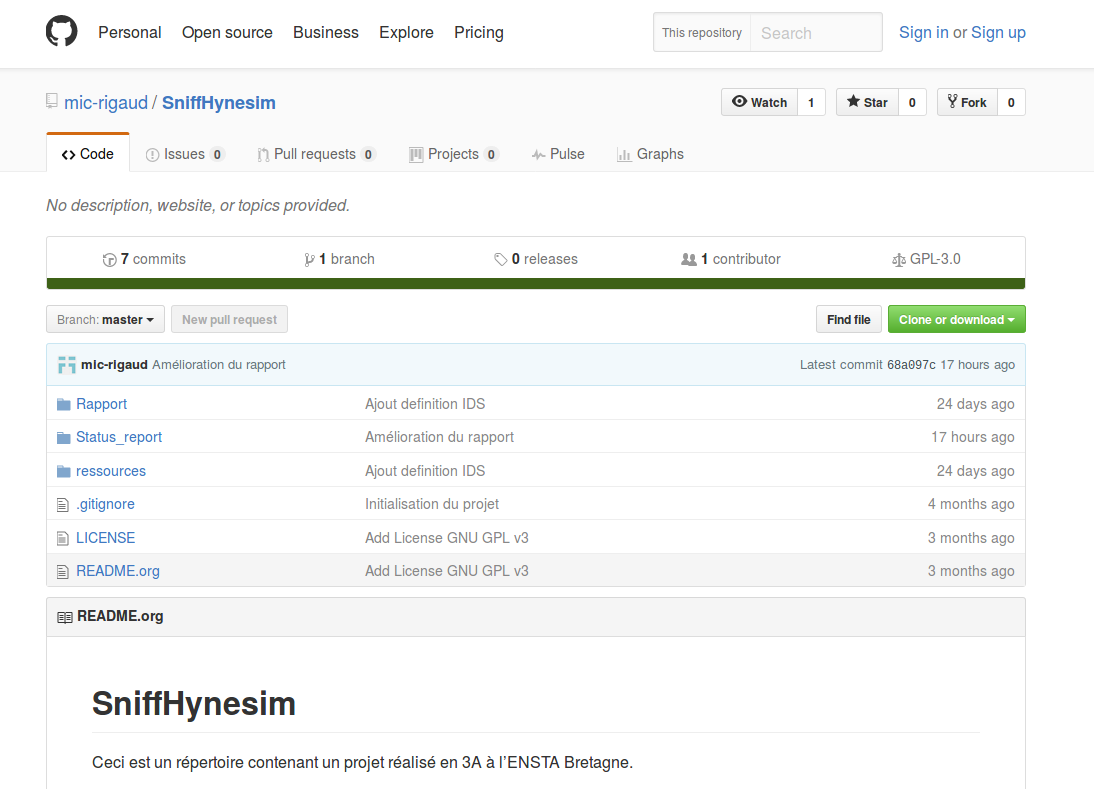
\includegraphics[width=\textwidth]{github}
  \caption{Github server}
  \label{fig:github}
\end{figure}

%%%%%%%%%%%%%%%%%%%%%%%%%%%%%%%%%%%%%%%%%%%%%%%%%%%%%%%%%%%%%%%%%%%%%%%%%%%%
%% TODO: Rajouter une image
%%%%%%%%%%%%%%%%%%%%%%%%%%%%%%%%%%%%%%%%%%%%%%%%%%%%%%%%%%%%%%%%%%%%%%%%%%%%



%%% Local Variables:
%%% mode: latex
%%% TeX-master: "../rapport_de_base"
%%% End:
